% métadonnées
\author{Paul, Hector KERVEGAN}
\title{Traitement et exploitation d'un corpus textuel semi-structuré: le cas des catalogues de vente de manuscrits.}
\date{05.09.2022}

% encodage, format, langue et police
\documentclass[a4paper, 12pt, twoside]{book}
\usepackage[english, french]{babel}
\usepackage[utf8x]{inputenc}
\usepackage[T1]{fontenc}
\usepackage{fontspec}
\usepackage{lmodern}
\usepackage{graphicx}

% code, graphiques et couleurs
\usepackage{minted}
\usemintedstyle{pastie}
\usepackage{tikz}
\usetikzlibrary{shapes.geometric}

% thx https://latexcolor.com/
\definecolor{palepink}{rgb}{0.98, 0.85, 0.87}
\definecolor{plum}{rgb}{0.44, 0.11, 0.11}
\definecolor{lilac}{rgb}{0.8, 0.8, 1.0}
\definecolor{peachpuff}{rgb}{1.0, 0.85, 0.73}
\definecolor{lightpink}{rgb}{1.0, 0.71, 0.76}
\definecolor{pearl}{rgb}{0.94, 0.92, 0.84}

% db interaction: db
% main step (start, stop...): main
% transfo/relation: transf
\tikzstyle{base} = [%
	draw,%
	rectangle,%
	rounded corners=3pt,%
	minimum height=1cm,%
	fill=lilac,%
	draw=plum,%
	text centered,%
	text width=4cm%
]
\tikzstyle{db} = [%
	cylinder,%
	shape border rotate=90,%
	aspect=0.25,%
	fill=peachpuff,%
	draw=plum,%
	text centered,%
	text width=4cm%
]
\tikzstyle{transf} = [%
	trapezium,%
	trapezium left angle=70,%
	trapezium right angle=110,%
	minimum height=1cm,%
	fill=lightpink,%
	draw=plum,%
	text centered,%
	text width=3cm%
]
\tikzstyle{choice} = [%
	diamond,%
	minimum width=2cm,%
	aspect=2,%
	fill=pearl,%
	draw=plum,%
	text centered,%
	text width=4cm%
]
\tikzstyle{arrow} = [%
	thick,%
	->,%
	>=stealth,%
	color=plum%	
]
\tikzstyle{line} = [%
	thick,%
	color=plum%	
]

% images
\usepackage{subcaption}

% mise en page ENC
\usepackage[margin=2.5cm]{geometry}
\usepackage{setspace}
\onehalfspacing
\setlength\parindent{1cm}

% bibliographie
\usepackage[toc]{appendix}
\usepackage{csquotes}
\usepackage[backend=biber,sorting=nyt,style=enc]{biblatex}
\nocite{*}
\addbibresource{bibliographie/visualisation.bib}
\addbibresource{bibliographie/katabase.bib}
\addbibresource{bibliographie/ecostat.bib}
\addbibresource{bibliographie/textprocessing.bib}
\defbibnote{intro}{Cette bibliographie contient tous les ressources utilisées pour l'écriture de ce mémoire.}

\DeclareSourcemap{%
 \maps[datatype=bibtex]{%
 	\map[overwrite]{%
 		\perdatasource{bibliographie/visualisation.bib}
 		\step[fieldset=keywords, fieldvalue={,visualisation}, append]
 	}
 	\map[overwrite]{%
 		\perdatasource{bibliographie/katabase.bib}
 		\step[fieldset=keywords, fieldvalue={,katabase}, append]
 	}
	\map[overwrite]{%
		\perdatasource{bibliographie/textprocessing.bib}
		\step[fieldset=keywords, fieldvalue={,text}, append]
	}
 	\map[overwrite]{%
 		\perdatasource{bibliographie/ecostat.bib}
 		\step[fieldset=keywords, fieldvalue={,econometrie}, append]
 	}
 }
}


% notes de bas de page, table des matières citations et index
\usepackage{imakeidx}
% \makeindex
% \makeindex[name=lieux,title=Index des noms de lieux]
\usepackage{tocbibind}

% autres paquets
\usepackage{ifthen}
 
% hyperref
\usepackage{hyperref}
\hypersetup{
 pdfauthor={Paul, Hector KERVEGAN}, 
 pdftitle={Traitement et exploitation d'un corpus textuel semi-structuré: le cas des catalogues de vente de manuscrits.}, 
 pdfsubject={Traitement de données textuelles},
 pdfkeywords={catalogues de vente}{mss}{katabase}{reconnaissance optique de caractères}{ocr}{web design}{visualisation de données}{traitement automatisé du language}{web de données}{Python}
}


% définition des acronymes
\usepackage[automake, acronym, toc]{glossaries}
\makeglossaries
\setacronymstyle{short-long}
% modèle: \newacronym{dom}{\textsc{dom}}{\emph{Document Object Model}}
% modèle bis: \newglossaryentry{meta}{name=métadonnée,description={donnée servant à définir ou décrire une autre donné quel que soit son support}}

% commandes perso: autres que les abbréviations
\newcommand{\scl}[1]{%
	% #1 : le siècle en chiffres romains
	#1%
	\ifthenelse{\equal{#1}{I}}{\up{er}}{\up{ème}}%
	~s.%
}

% commandes perso: abréviations
% technologies en mono, sigles et sites web en italique
\newcommand{\api}{\texttt{API}}
\newcommand{\alto}{\texttt{Alto}}
\newcommand{\escr}{\textit{eScriptorium}}
\newcommand{\html}{\texttt{HTML}}
\newcommand{\js}{\texttt{Javascript}}
\newcommand{\json}{\texttt{JSON}}
\newcommand{\ktb}{\textit{Katabase}}
\newcommand{\mss}{\textit{MSS}}
\newcommand{\mssktb}{\mss{} / \ktb{}}
\newcommand{\py}{\texttt{Python}}
\newcommand{\rgx}{\textit{expressions régulières}}
\newcommand{\rdf}{\texttt{RDF}}
\newcommand{\sparql}{\texttt{SPARQL}}
\newcommand{\tei}{\texttt{TEI}}

\newcommand{\titem}{\texttt{item}}
\newcommand{\tname}{\texttt{name}}
\newcommand{\tnum}{\texttt{num}}
\newcommand{\ttrait}{\texttt{trait}}
\newcommand{\tp}{\texttt{p}}
\newcommand{\tdesc}{\texttt{desc}}
\newcommand{\tdate}{\texttt{date}}
\newcommand{\tmeasure}{\texttt{measure}}
\newcommand{\tnote}{\texttt{note}}

\newcommand{\xml}{\texttt{XML}}
\newcommand{\xmltei}{\texttt{XML-TEI}}
\newcommand{\xsl}{\texttt{XSL}}
\newcommand{\wkd}{\textit{Wikidata}}

% modèle: https://www.overleaf.com/project/61a6185ee83481070ab68d99
% liste des mémoires: https://docs.google.com/spreadsheets/d/1CZRaEX4BMqHNtqr97Dhg9UV9bPTt_4XS_IgPL5A-ZbU/edit


%%%%%%%%%%%%%%%%%%%%%%%%%%%% DÉBUT %%%%%%%%%%%%%%%%%%%%%%%%%%%
\begin{document}
	\onehalfspacing
	
	\begin{titlepage}
		\begin{center}		
			\bigskip
			
			\begin{large}
				ÉCOLE NATIONALE DES CHARTES\\
			\end{large}
			
			\rule{2cm}{0.02cm}
			
			\begin{Large}
				\textbf{Paul, Hector Kervegan}\\
			\end{Large}
			
			\vfill
			
			\begin{Huge}
				\textbf{Traitement, exploitation et analyse d'un corpus semi-structuré: le cas des catalogues de vente de manuscrits}
			\end{Huge}
			
			\vfill
			
			\begin{large}
				Mémoire pour le diplôme de master \\
				\emph{Technologies numériques appliquées à l'histoire}
				
				\bigskip
				
				2022
			\end{large}
			
		\end{center}
	\end{titlepage}

\frontmatter
\chapter*{Résumé}
\addcontentsline{toc}{chapter}{Résumé}

\mainmatter
\chapter*{Introduction}
\addcontentsline{toc}{chapter}{Introduction}
J'ai choisi de structurer mon mémoire autour de plusieurs questions connexes, qui, à différents degrés, se retrouvent tout au long du développement:

En quoi la nature semi-structurée du corpus permet d'en automatiser le traitement? Comment produire des informations normalisées et exploitables à partir d'un corpus textuel semi-structuré ? En quoi ce traitement et la traduction des documents vers d'autres formats et d'autres médias impacte leur réception ? Quels sont les choix techniques qui influencent cette réception ?

Les deux premières questions, d'orientation plutôt technique, forment la colonne vertébrale pour le mémoire; elles lient deux aspects centraux: la nature du corpus et la manière dont sa structure permet toute la chaîne de traitement. Par \enquote{semi-structuré}, j'entends que, à un niveau distant, toutes les entrées de catalogue suivent la même structure; des séparateurs distinguent les différentes parties, et les informations sont souvent structurées de manière semblable pour chaque manuscrit vendu. Cela permet un traitement de \enquote{basse technologie} (\emph{low-tech}) en évitant d'entraîner de lourds modèles de traitement du langage naturel (ce qui aboutirait à des solutions complexes, difficiles à maintenir et à faire évoluer et relativement opaques dans leur fonctionnement). À l'inverse, un corpus semi-structuré peut être traité en déduisant une \enquote{structure abstraite}, que chaque entrée de catalogue partage. Il est alors possible de mettre en place des solutions techniques plus faciles, pour un résultat de qualité équivalente. Produire des \enquote{informations normalisées et exploitables} implique de traiter le corpus en cherchant des réponses à des questions de recherche précises -- dans le cadre de mon stage, une question centrale a été de chercher à isoler les facteurs déterminant le prix d'un manuscrit.

Les deux dernières questions, au premier abord plus théoriques, me semblent centrales, notamment à la troisième partie de ce mémoire. Numérisation, traitement informatisé et diffusion sur le web ne sont pas des opérations neutres, mais un ensemble de \enquote{traductions} des documents originels. Ces processus comportent une part de choix conscients, qu'il s'agit de mettre en avant. Par exemple, on considère que la majorité des documents vendus ont pour titre l'auteur.ice du document. Cette personne n'est cependant pas toujours mentionnée, et des documents peuvent être nommés d'après un lieu, un évènement ou un thème (la Révolution française, par exemple). Ces \enquote{traductions} des catalogues sont relativement discrètes tout au long de la chaîne de traitement (où le format dominant est la \tei{}, qui garde une relation d'équivalence avec le texte). C'est lors du  passage au site web que ce processus de traduction devient plus évident, et, potentiellement, plus problématique. On y abandonne la référence au document originel (les catalogues numérisés ne sont pas accessibles en ligne par un.e utilisateur.ice), le catalogue n'est plus la manière privilégiée d'accéder aux items vendus... De plus, la construction d'un site web implique la conception d'une interface et, dans notre cas, la production d'une série de visualisations intégrées au site. Le passage au site web remet aussi en cause la hiérarchie habituelle entre ingénierie et recherche: la conception d'un site ne répond pas à une question scientifique, mais elle soulève ses propres questions. Loin d'être anodines, ces problématiques de design déterminent la construction et la réception des savoirs. Il est donc important, je pense, de problématiser ces questions de visualisation et de design.




%%%%%%%%%%%%%%%%%%%%%%% PREMIÈRE PARTIE %%%%%%%%%%%%%%%%%%%%%%
\part{Du document numérisé au \xmltei: nature du corpus, structure des documents et méthode de production des données}
\chapter{Le marché des manuscrits autographes au prisme des catalogues de vente}
\chaptermark{Le marché des manuscrits autographes}
Ce chapitre présente l'objet d'étude du projet \mss{} : étudier le marché des manuscrits autographes du \scl{XIX}. parisien à partir de ses catalogues de vente et étudier la construction du canon littéraire au prisme du marché du manuscrit.

\section{Pourquoi étudier le marché des manuscrits autographes?}
Cette section porte sur l'intérêt scientifique des objets d'étude du projet (marché des manuscrits et étude de la construction du canon).


\section{La structure du corpus : périodisation, producteurs des documents et classification}
Ici est faite une présentation des documents traités dans le cadre du projet MSS. La présentation est à deux niveaux: au niveau du corpus et des catalogues. Ce chapitre s'appuie sur les mémoires effectués par d'ancien.ne.s stagiaires de \ktb{}, qui ont déjà beaucoup analysé la nature et les enjeux du corpus\footcite{rondeau_du_noyer_encoder_2019, corbieres_du_2020, janes_du_2021}.

\subsection{Le corpus de catalogues de vente de manuscrits}
Ici est présenté le corpus: nature, quantité de documents (et d'entrées individuelles), dates, différentes classifications qui peuvent être faites (revues, catalogues de ventes aux enchères ou à prix fixes...).

\subsection{Structure des catalogues}
Ici sera présentée la structure des catalogues; la structure de chaque page ne sera détaillée qu'à la partie suivante.


\chapter{Production des données: de l'OCR à la \tei{}}
\chaptermark{Production des données}
Cette partie s'attache autant à présenter le processus d'océrisation (qui est déjà bien établi et ne constitue pas le cœur de mon stage) que la structure des documents. Alors que le chapitre précédent s'intéresse aux catalogues dans leur ensemble, ici, on étudie le corpus au niveau de la page et de l'entrée individuelle. En effet, l'océrisation repose sur la segmentation, et donc sur l'établissement d'une structure \enquote{abstraite} d'une page (c'est-à-dire, d'un découpage de la page en zones).

\section{Extraire le texte des imprimés}
\subsection{Comprendre la structure du document pour préparer l'édition numérique}

\subsubsection{Appréhender la structure de la page à l'aide de SegmOnto}
La structure des catalogues est présentée au niveau de la page. L'ontologie SegmOnto\footcite{christensen_segmonto_2022} est utilisée, autant pour appréhender la structure de la page que pour exprimer cette structure de façon standardisée.

\subsubsection{Description des entrées de catalogue: préparer l'édition \tei{}}
Ici, la structure des catalogues est présentée au niveau de l'entrée, c'est à dire du lot mis en vente. C'est à autour de la structure des entrées qu'est construite l'édition \xmltei{}. On s'intéresse à la structure des entrées individuelles à deux niveaux:
\begin{itemize}
	\item Au niveau intellectuel: quelles sont les différentes parties d'une entrée (titre, description du manuscrit, prix...).
	\item Au niveau  \enquote{textuel}: quels sont les séparateurs, c'est à dire les éléments dans le texte qui permettent de séparer les pages de catalogue en entrées et les entrées en sous-éléments) correspondant à la structure intellectuelle décrite ci-dessus.
\end{itemize}

\section{L'encodage des manuscrits en \xmltei{}}
\subsection{Encoder les catalogues en \tei{}}
Ici est présentée la représentation \xmltei{} des catalogues de vente.

\subsection{L'encodage en \tei{}: un processus sélectif qui réduit les significations du texte}
Après une étape d'océrisation via \escr{}, le texte extrait des PDF peut être exporté soit en texte brut, soit en \xml{} \texttt{Page} ou \alto{}. Ces formats s'attachent à garder une relation entre le \xml{} et le document numérisé (les zones de texte sont indiquées, chaque ligne est dans une balise...). Cependant, l'unité intellectuelle centrale à la suite du projet, ce n'est pas la page numérisée, mais l'entrée de catalogue. Un format plus complexe que le \xml{} d'\escr{} est donc nécessaire. Assez logiquement, la suite du projet s'appuie sur une traduction des catalogues en \tei{}. On s'intéresse autant à la structure des documents \xml{} (quelles balises sont utilisées...) qu'à l'intérêt scientifique d'une édition numérique (balisage sémantique, possibilité de normaliser les informations grâce à des attributs).

L'édition numérique en \xmltei{} des catalogues implique une certaine perte d'informations: l'intégralité des significations contenues dans les catalogues imprimés ne peut être traduite en \tei{} (la police, ou la qualité du papier, peuvent être documentés mais ne peuvent pas être reproduites). Ce genre de perte d'information a lieu, à différents degrés, dans la plupart des éditions \tei{}: ce format n'est pas un substitut des documents originels. Dans le projet \mssktb{}, d'autres informations sont perdues: l'édition numérique n'est pas censée être une représentation exhaustive des catalogues. La \tei{} n'est pas utilisée comme un format de conservation, mais comme un format de traitement qui sera enrichi dans les différentes étapes. Afin de mesurer ce qui est conservé et ce qui est perdu du document originel, l'édition \tei{} sera analysée à la lumière de la \enquote{roue du texte} du philologue Patrick Sahle\footcite[p. 11]{sahle_digital_2016} qui modélise les significations plurielles d'un texte.

John Frow + Susan Pearce ?


%%%%%%%%%%%%%%%%%%%%%%% DEUXIEME PARTIE %%%%%%%%%%%%%%%%%%%%%%
\part{Normalisation, enrichissements et extraction d'informations: une chaîne de traitement pour des données semi-structurées}

\chapter{Faire sens d'un corpus complexe: homogénéisation des données et extraction d'informations}
\chaptermark{Faire sens d'un corpus complexe}

\section{Homogénéiser et normaliser un corpus complexe}
Cette section s'intéresse à la manière dont les fichiers \tei{} sont traités afin de pouvoir ensuite en extraire des informations. C'est directement grâce la structure des entrées (et grâce à la nature \enquote{semi-structurée} des catalogues) qu'est possible le traitement automatisé des documents.

\subsection{Pourquoi chercher à normaliser le corpus?}
La question mérite d'être posée: des étapes de post-traitement du corpus sont nécessaires pour pouvoir en extraire des informations et pour pouvoir donc en faire sens; cependant ce processus peut également impacter la nature du texte et ses significations. Tout comme l'édition \tei{} originelle est un processus sélectif, le traitement des documents encodés est lui un processus sélectif: certaines informations contenues par l'encodage sont privilégiées aux dépens d'autres. Il s'agit ici d'expliciter ces choix (travailler sur les prix, les formats et dimensions des manuscrits plutôt que sur leur sujet) et de les justifier. Cette section s'attache donc à rappeler les questions de recherche qui sous-tendent la normalisation des documents (ajouter plus de structure au document \tei{} pour l'exploiter plus facilement, uniformiser la notation des tailles et des dimensions des documents...).

\subsection{Comment normaliser le corpus tout en préservant sa valeur documentaire?}
Ici, on s'intéresse à la manière dont la \tei{} est mise à profit pour enrichir le corpus tout en conservant le contenu textuel des catalogues. Les différentes étapes de normalisation sont également rappelées (ce travail n'étant pas au cœur de mon stage, il s'agira plutôt d'un rappel que d'une présentation technique détaillée).

\section{Faire sens du corpus: extraction d'informations et fouille de texte}
Ici sont décrits le processus et les objectifs de l'extraction d'informations à partir des fichiers \tei{}. C'est à partir de cette opération d'extraction que sont construites les visualisations, qui permettent une approche graphique du corpus et une meilleure compréhension de celui-ci.

\subsection{Extraire des informations au niveau des entrées}
Des données sont extraites pour chaque entrée de catalogue (un travail largement effectué par A. Bartz, que j'ai légèrement mis à jour) : prix (dans la monnaie de l'époque et en francs constants), date de vente normalisée, nom de l'auteur.ice et description du manuscrit... L'extraction d'informations pour les entrées individuelles permet surtout de faire une réconciliation des manuscrits vendus (c'est à dire, de retrouver les items vendus plusieurs fois).

\subsection{Extraire des informations au niveau des catalogues}
Un second processus d'extraction produit des données pour chaque catalogue de vente: titre du catalogue, date de vente, nombre d'items vendus, prix minimum, inférieur et maximum, prix moyen et médian, variance... Ce processus met l'accent sur une approche statistique et économique du corpus, qui permettra d'étudier l'évolution du cours et du volume du marché des manuscrits (nombre d'items en vente, évolution des prix).

\subsection{Vers une approche économique du corpus: la conversion automatique des prix en francs constants}
En même temps que ces processus d'extraction d'informations, un script de conversion des monnaies (françaises et étrangères) en francs constants 1900 a été élaboré. En annulant l'effet de l'inflation, les francs constant permettent d'étudier l'évolution réelle des prix.


\chapter{Vers une étude des facteurs déterminant le prix des documents: alignement des entrées du catalogue avec \wkd{} et exploitation de données normalisées}
\chaptermark{Vers une étude...}
Ce chapitre est construit autour d'une question de recherche: comment produire des informations exploitables pour une étude économétrique à partir d'un corpus textuel semi-structuré? Un des objectifs du projet est de faire l'étude des facteurs déterminant le prix d'un manuscrit. Pour faire cette étude, il faut obtenir, pour chaque entrée du catalogue, un certain nombre d'informations normalisées. Le travail d'extraction de données présentes dans les catalogues a déjà été fait par de précédent.e.s stagiaires. Ces données sont principalement quantitatives: prix des manuscrits, dimensions et nombre de pages, date de création. Il est nécessaire de compléter les informations par des données qualitatives et d'enrichir les données disponibles avec des sources extérieures. Pour ce faire, il a été choisi d'aligner le nom des auteur.ice.s des manuscrits avec des identifiants \wkd{}; dès lors que l'on a un identifiant \wkd{}, il est possible de récupérer automatiquement des informations sur les personnes via \sparql. Le choix de travailler uniquement sur les noms, et non sur la description des documents, a deux motivations:
\begin{itemize}
	\item Les noms de personnes (et la manière dont elles sont décrites) constituent la partie la plus normalisée des documents. La description des manuscrits est plutôt en \enquote{texte libre}. Dans la continuité avec le reste du projet, nous sommes resté dans une approche \enquote{basse technologie}, qui consiste à s'appuyer majoritairement sur des solutions techniquement simples. C'est pourquoi nous avons préférer traiter les noms avec des tables de correspondance\footnote{C'est à dire, des tables qui permettent de normaliser la manière dont les informations figurent dans les catalogues, et donc de remplacer des termes \enquote{vernaculaires} par leurs équivalents utilisés par \wkd{}} et des \rgx{}, plutôt que de faire du TAL sur la description des documents.
	\item Toutes les informations \enquote{simples} (données quantitatives facilement normalisables: dates etc.) ont déjà été extraites des descriptions des manuscrits.
\end{itemize}

Ce travail d'enrichissement a été fait en deux temps. 

La première étape, et la plus difficile, est l'alignement avec \wkd{}. Cela demande d'extraire un ensemble d'informations à partir du nom de la personne et de la description de celle-ci. Parmi les informations extraites: nom, prénom, titre de noblesse, occupation, dates de vie et de mort. À partir de ces informations, stockées dans un dictionnaire, un algorithme construit successivement différentes chaînes de caractères pour lancer des recherchers en plein texte sur l'\api{} de \wkd{}. L'objectif est que le premier résultat recherché sur \wkd{} soit correct. Sur un jeu de test, le score F1 \footnote{Le score F1, ou \textit{F-score}, est la moyenne harmonique de la précision (vrais positifs par rapport au total de résultats obtenus) et du rappel (nombre de résultats positifs par rapport au total de résultats positifs).\cite{noauthor_precision_2022}} obtenu est de 68\%. Un relecture \enquote{manuelle} des résultats est donc nécessaire.

La deuxième étape, nettement plus simple, consiste à lancer des requêtes \wkd{} sur les identifiants récupérés afin de récupérer des informations sur les auteur.ice.s des manuscrits (cette partie du travail est encore en cours) pour enrichir nos données.

Une fois ce travail effectué, l'enrichissement des données à proprement parler est possible: les fichiers \tei{} sont mis à jour pour ajouter les identifiants \wkd{}. Ainsi, il est possible de faire le lien entre les entrées de catalogues dans des fichiers \xml{} et les données issues de requêtes \sparql{}, stockées dans un \json.


\section{Questions introductives: pourquoi et comment s'aligner avec \wkd{} ?}
\chaptermark{Questions introductives}
Cette section, introductive, répond à des questions évidentes mais essentielles: elles permettent de mettre au clair l'intérêt et les (multiples) difficultés dans l'alignement avec \wkd{}.

\subsection{Pourquoi s'aligner avec des identifiants \wkd{}?} 
% Nos données sont déjà complètes, une pipeline entière existe déjà. Cependant, il peut être difficile de déterminer ce qui fait le prix d'un manuscrit. On aborde les manuscrits avec nos propres catégories intellectuelles du \scl{XXI}, et notre connaissance de l'histoire de l'époque. Il n'est pas non plus possible de reconstruire d'une manière exacte le regard qu'un public du \scl{XIX} aurait sur ces manuscrits -- ce qui permettait de revenir à une perception antérieure de la valeur. Il faut donc chercher à contourner ces biais en produisant des données aussi objectives que possibles. Ainsi, un maximum de variables sont à notre disposition pour calculer des régressions linéaires (qui permettent de prédire l'impact d'une variable sur l'évolution des prix).

L'alignement avec \wkd{} a pour objectif principal de mieux comprendre les déterminants du prix des manuscrits sur le marché du \scl{XIX}. Mais pourquoi passer par un alignement avec \wkd{}? 

Pour étudier les déterminants du prix d'un manuscrit, il faut établir la relation entre la variable dont la valeur est étudiée (le prix d'un manuscrit) et un ensemble d'autres facteurs (qui a écrit un manuscrit, quelles sont ses dimensions, de quand date le document...). En d'autres termes, il faut étudier le comportement d'une variable en fonction d'autres variables. En économétrie, cette opération s'appelle le calcul de régressions linéaires. La variable étudiée (le prix) est dite la variable expliquée; les facteurs déterminant la valeur de cette variable sont dites \enquote{variables explicatives}\footcite{noauthor_regression_2022}. Cependant, cette opération est loin d'être anodine: il faut d'abord identifier les variables pertinentes, et ensuite trouver un moyen de les quantifier. Deux difficultés se présentent pour alors.

Premièrement, il faut pouvoir quantifier les variables expliquées pour calculer des régressions linéaires. Il est possible de leur assigner une valeur numéraire (ce qui est aisé pour les informations quantitatives des catalogues: la date de l'écriture d'un manuscrit, ses les dimensions). Une autre possibilité est de quantifier la présence ou non d'une variable: mention d'un.e destinataire ou du contenu d'un manuscrit. Cependant, ces approches quantitatives ne permettent pas de quantifier des informations complexes, comme la célébrité des auteur.ice.s, ou encore si un manuscrit porte sur un évènement historique ou biographique important (le manuscrit d'un texte célèbre, par exemple, pourrait avoir une valeur particulières). Ces informations sont parfois être présentes dans les catalogues; elles peuvent aussi être connues des lecteur.ice.s d'aujourd'hui et des acheteurs et acheteuses de l'époque. Il n'existe cependant pas de méthodes faciles pour détecter ou quantifier la célébrité d'une personne, ou l'importance d'un sujet.

Une deuxième difficulté découle justement de la part d'implicite qu'il y a dans les catalogues. Les descriptions des items vendus sont brèves, et comprendre ce qui fait la valeur d'un manuscrit demande aux acheteur.euse.s d'avoir des références culturelles et historiques: celles-ci permettent d'identifier l'auteur.ice ou le sujet, et donc pour comprendre la valeur d'un manuscrit. Dans le cadre du projet \mssktb{}, les entrées de catalogues sont traitées par une machine qui, en toute logique, ne dispose pas de ces références. La compréhension qualitative des entrées de catalogues n'est donc pas compatible avec l'approche par lecture distante du projet. Pour éviter de perdre ces informations qualitatives essentielles, il est donc nécessaire de trouver un moyen de quantifier le qualitatif.

En bref, la question est: comment faire la différence entre une lettre de La Rochefoucauld (\ref{fig:rochefoucauld}), vendue 200 francs, et la deuxième (\ref{fig:villars}), vendue à 30 francs? Le problème est un problème de lecture. Une observation de la description des lettres par un être humain comme par une machine peuvent identifier des éléments semblables dans le texte: les deux lettres sont écrites par des ducs; l'une est une \enquote{Très-belle lettre} (\ref{fig:rochefoucauld}), l'autre est une \enquote{Lettre intéressante} (\ref{fig:villars})\footnote{Ce sont des informations qui se retrouvent souvent, et il est donc possible d'écrire un programme qui les relève automatiquement}. Bien que les lettres partagent des attributs, il y a une forte différence de prix entre les deux manuscrits. Un.e lecteur.ice peut trouver une raison à cette différence de prix: La Rochefoucauld et Madeleine de Scudéry n'ont pas le même statut que le duc de Villars. Un regard humain peut donc interpréter un prix et déterminer une valeur en s'appuyant sur ses connaissances. La lecture est qualitative et s'appuie sur de l'implicite, ce qui n'est pas possible pour une machine: formellement, rien ne distingue un nom d'un autre; lorsqu'un programme \enquote{lit} un texte, il ne peut pas s'appuyer sur ses connaissances pour déterminer ce qu'un nom signifie, ce à quoi il fait référence.

\begin{figure}[h!]
	\centering
	\begin{subfigure}{0.8\textwidth}
		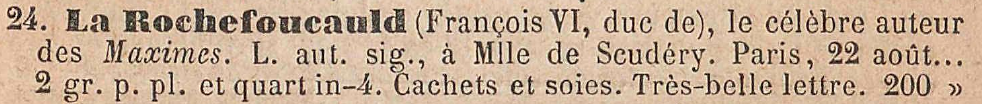
\includegraphics[width=\textwidth]{img/cat_000372_e24.png}
		\caption{Une lettre écrite par La Rochefoucauld vendue à 200 francs.}
		\label{fig:rochefoucauld}
	\end{subfigure}
	\begin{subfigure}{0.8\textwidth}
		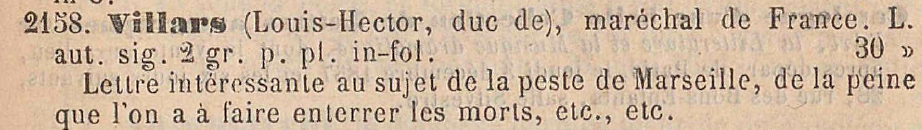
\includegraphics[width=\textwidth]{img/cat_000382_e2158.png}
		\caption{Une lettre écrite par Louis-Hector Villars vendue à 30 francs.}
		\label{fig:villars}
	\end{subfigure}
	\caption{Deux exemples de lettres}
\end{figure}

Pour analyser efficacement la variable \enquote{prix}, il faut pourtant pouvoir, dans une certaine mesure, comprendre les informations implicites et qualitatives contenues dans les catalogues. Le parti pris a donc été de construire le socle de connaissance qui manque à une machine, en s'alignant avec \wkd{} et en s'en servant pour enrichir nos données. Le choix a été fait de ne s'aligner avec \wkd{} que pour certaines parties des entrées de catalogue. Pour rappel, voici leur structure:

\inputminted[linenos, breaklines, tabsize=4]{xml}{code/tei_item.xml}

Les entrées de catalogue contiennent beaucoup d'informations qualitatives, qui pourraient avoir une influence sur le prix du manuscrit: ici par exemple, la description du contenu de la lettre dans le \tnote{}; il est également souvent fait mention du ou de la destinataire. Cependant, l'alignement avec \wkd{} n'a pas été fait avec l'intégralité des entrées. C'est seulement le contenu du \tname{} qui a été aligné avec \wkd{}, à l'aide des informations contenues dans le \ttrait{}. Le \tdesc{} a déjà fait l'objet d'un grand travail de normalisation et d'extraction d'informations; un alignement avec des sources externes n'aurait donc pas une très grande plus-value. L'élément \tnote{} contient souvent des informations intéressantes, puisque c'est là qu'est décrit le contenu d'un manuscrit. Cependant, cet élément n'est pas toujours présent; son contenu est souvent écrit en langage naturel, non structuré, et contient des informations trop variées pour développer un traitement uniforme. Il est donc difficile de tirer parti de cet élément. Le \tname{} et son \ttrait{} sont les éléments les plus régulièrement présents; les informations qu'ils contiennent sont toujours les mêmes (nom d'une personne ou thème d'un manuscrit dans le \tname{}, description du \tname{} dans le \ttrait{}); enfin, ces deux éléments n'ont pas du tout été transformés dans le reste de la chaîne de traitement. Ils portent donc des informations qualitatives centrales pour produire des données exploitables dans une étude économétrique.

Le parti pris a donc été d'aligner avec des identifiants \wkd{} les noms contenus dans les balises \tname{} à l'aide des descriptions contenues dans les \ttrait{}; à partir de cet alignement a été constituée une base de données. Cela permet d'approximer une lecture \enquote{humaine} des items en vente: pour chaque auteur.ice, un certain nombre d'informations auront été récupérées pour mieux identifier la personne (ses occupations, son origine, ses dates de vie...). L'analyse du corpus s'appuit alors sur un bagage de connaissances qui permet d'appréhender par lecture distante l'importance d'une personne. Il devient alors envisageable de voir dans quelle mesure la mention d'une personne impacte le prix d'un manuscrit, et quels sont les facteurs biographiques déterminant dans l'établissement de la valeur. Pour revenir à l'exemple de La Rochefoucauld: à défaut de permettre de savoir qui il est, un alignement avec \wkd{} permet d'identifier son statut et sa place dans la culture française, en récupérant le nombre de ses publications ou encore les institutions dont il est membre.


\subsection{Présentation générale de l'algorithme}
À l'aide d'un schéma, on présente l'intégralité de la \textit{pipeline} pour cette étape: préparation des données; lancement des recherches en plein texte sur l'\api{} \wkd{}; lancement de requêtes \sparql{} à partir des résultats obtenus et structuration des résultats.

\begin{figure}[!h]
	\centering
	\tikz[node distance=1cm, scale=0.9, transform shape]{
		\node[db] %
			(db1) at (-5,0)%
			{Source: tableur contenant les \tname{} et \titem{}};
		\node[base]%
			(start) at (0,0)%
			{Lancement de l'algorithme sur toutes les entrées du tableur};
		\draw[arrow] (db1) -- (start);
		
		\node[choice]%
			(detect) at (0,-3.5)%
			{Détection du type de \tname{} pour établir %
				la méthode d'extraction des données};
		\draw[arrow] (start) -- (detect);
		
		\node[transf]%
			(name) at (-4,-6.5)%
			{Extraction et normalisation d'informations nominatives du \tname{}};
		\node[transf]%
			(trait) at (4,-6.5)%
			{Extraction et normalisation d'informations biographiques du \ttrait{}};
		\node[base]%
			(dict) at (0,-9.5)%
			{Constitution d'un dictionnaire structuré pour aligner les \tname{} avec des entités \wkd{}};
		\draw[arrow] (detect) -- (name);
		\draw[arrow] (detect) -- (trait);
		\draw[arrow] (name) -- (dict);
		\draw[arrow] (trait) -- (dict);
		
		\node[db]%
			(logs) at (5,-11.5)%
			{Optimisation: enregistrement des entrées de catalogues déjà et requêtes déjà traitées};
		\node[transf]%
			(api) at (0,-13)%
			{Alogrithme de requêtes sur l'API \wkd{} pour récupérer des identifiants};
		\draw[arrow] (dict) -- (logs);
		\draw[arrow] (api) -- (logs);
		\draw[arrow] (dict) -- (api);
		
		\node[db]%
			(idset) at (0,-17.5)%
			{Liste d'identifiants \wkd{} à partir de laquelle est constitué le jeu de données};
		\node[transf]
			(sparql) at (0,-20)
			{Requêtes \sparql{}};
		\node[db]%
			(sparqldata) at (0,-23)%
			{Jeu de données issues de \sparql{} enregistré en \json{}};
		\draw[arrow] (api) -- (idset);
		\draw[arrow] (idset) -- (sparql);
		\draw[arrow] (sparql) -- (sparqldata);
	}
	\caption Présentation générale de l'algorithme d'enrichissement de données via \wkd{}
	\label{fig:wkdmain}
\end{figure}


\subsection{Quelles données rechercher via \sparql?}
Après avoir expliqué pourquoi développer des méthodes d'enrichissement automatique, une seconde question se pose: quelles sont les données à récupérer? Cette question n'est pas anodine du fait de la diversité du corpus. Le titre donné à un manuscrit dans un catalogue et inscrit dans le \tname{} est souvent celui d'une personne, mais ce n'est pas toujours le cas. Il arrive également qu'un manuscrit soit nommé d'après un évènement (la Révolution française), un lieu ou une province (Italie, Poitou), ou encore une typologie de document (des chartes).

Un bref retour sur la manière dont fonctionne \sparql{} permet de mieux comprendre le problème que peut poser la diversité du corpus. \sparql{} a l'avantage de permettre de récupérer des données propres sur des bases de données en ligne; cependant, l'information y est organisée de manière très spécifique, ce qui demande de faire des requêtes précises. Ce langage de requêtes a pour but d'interagir avec une base de données au format \rdf{}. Avec ce format -- dit sémantique -- les données sont organisées en \enquote{triplets} sujet--prédicat--objet, où:

\begin{itemize}
	\item le sujet est la ressource principale.
	\item le prédicat est une propriété du sujet, qui caractérise une relation avec une autre ressource, l'objet.
	\item l'objet est une ressource secondaire: c'est la valeur d'un prédicat.
\end{itemize}

Le principe des triplets \rdf{} est mieux exprimé sous forme graphique (\ref{fig:triplet}):

\begin{figure}[!h]
	\centering
	\tikz{
		\node%
			[base] %
			(S) at (0,0) %
			{\textbf{Sujet} \small \\ La ressource principale \\ \textit{Natalia Gontcharova}};
		\node%
			[transf] %
			(P) at (5, 0) %
			{\textbf{Prédicat} \small \\ La relation à l'objet \\ \textit{a peint}};
		\node%
			[base] %
			(O) at (10, 0) %
			{\textbf{Objet} \small \\ Une ressource secondaire \\ \enquote{\textit{Les porteuses}}};
			
		\draw[arrow] (S) -- (P);
		\draw[arrow] (P) -- (O);
	}
	\caption{Exemple de relation sujet -- prédicat -- object}
	\label{fig:triplet}
\end{figure}

Deux particularités supplémentaires définissent les formats sémantiques:
\begin{itemize}
	\item Toutes les \enquote{ressources} peuvent être tour à tour sujet ou objet. L'exemple du dessus, par exemple, aurait pu être réécrit sous la forme: \enquote{Les porteuses} a été peint par Natalia Gontcharova. Dans ce cas, Natalia Gontcharova est l'objet et \textit{Les porteuses} est le sujet. Par conséquent, une base de données \rdf{} est une base de donnée en graphes; elle peut être représentée sous la forme d'un réseau de ressources qui entretiennent des relations bilatérales entre elles. Il n'y a pas de hiérarchie entre les informations, contrairement à une base de données \xml{} classique.
	\item L'ensemble des ressources et des prédicats d'une base de donnée en graphe sont définis et disposent d'un identifiant unique. Les prédicats, plus particulièrement, sont définis selon une ontologie particulière.
\end{itemize}

Le deuxième point complexifie la définition des données à récupérer via \sparql{}: les prédicats sont décrits avec une grande précision; par conséquent, une information analogue peut être représentée par différents prédicats dans différentes situations. Dans l'ontologie \wkd{}, la création d'un texte et la création d'une peinture ne correspondent pas au même prédicat. Pour que les données soient utilisables, il faut être très spécifique quant aux informations recherchées. 

Les 18899 entités avec lesquelles les entrées de manuscrits ont été alignées peuvent se classer en de nombreuses catégories. Sur \wkd{}, une entité est une \enquote{instance} d'une classe plus large. En suivant la classification de \wkd{}, les entités appartiennent aux catégories suivantes\footnote{Un graphique présentant l'ensemble de ces catégories se trouve en annexes (\ref{appendix:wikidata_instances}).}:
\begin{itemize}
	\item personnes humaines; cette catégorie est la plus fréquente (12090 occurrences)
	\item noms de familles (3180 entités)
	\item communes françaises (586 occurrences)
	\item peintures et sculptures (respectivement 520 et 236 entités)
\end{itemize}

Cette variété peut s'expliquer en partie par le taux d'erreur dans l'alignement avec Wikidata. Cependant, toutes ces \enquote{erreurs} ne correspondent pas forcément à des résultats qui ne sont pas pertinents. Par exemple, l'algorithme peut aligner un.e écrivain.e avec un de ses ouvrages, ou une personne avec son portrait. Des résultats erronés peuvent toujours garder une forme de pertinence. Il est d'autant plus important de construire des requêtes \sparql{} qui se concentrent pas uniquement sur des personnes. Cependant, il n'est pas possible de faire une requête qui correspondent à toutes les catégories auxquelles appartiennent le corpus. Le choix a donc été fait de se concentrer sur les catégories les plus pertinentes: les personnes, les familles, et les œuvres artistiques et littéraires. Non seulement ces catégories contiennent la grande majorité du corpus (16026 entités), mais ces catégories sont les plus à même de contenir des entités pertinentes. Il a été choisi de ne pas faire de requête spécifique sur les lieux, puisque peu d'informations sont disponibles pour les entités de la catégorie \enquote{communes françaises} sur Wikidata.

Un nombre assez conséquent de données ont donc été requêtées avec \sparql{}, du fait des spécificités des bases de données en graphes, de la variété des entités \wkd{} auxquelles les manuscrits sont liées, et enfin du fait de la variété du corpus lui même. Ces informations récupérées correspondent aux différentes catégories de \wkd{}.
\begin{itemize}
	\item Pour les personnes et les familles, les informations suivantes sont récupérées sur \wkd{}:
	\begin{itemize}
		\item Le genre de la personne;
		\item Sa nationalité, afin de voir si l'origine d'une personne influence le prix d'un manuscrit;
		\item Les langues parlées par une personne; là encore, l'objectif est d'étudier l'impact de l'origine d'un.e auteur.ice sur un prix.
		\item Les date de vie et de mort, afin de placer un manuscrit dans une époque et de voir comment son ancienneté et sa contemporanéité en influencent le prix.
		\item Le lieu où une personne est née, où elle a vécu et où elle est morte, pour des raisons analogues.
		\item La manière dont la personne est morte. Si cette information peut sembler anecdotique à un public contemporain, les catalogues de ventes sont marqués par un goût du sensationnel, et la manière dont une personne est morte est souvent mentionnée, notamment en cas d'exécutions.
		\item La religion d'une personne: il peut être intéressant d'étudier si, et comment, ce critère influence l'évolution d'un prix.
		\item Les titres de noblesse d'une personne.
		\item L'éducation qu'a reçu une personne, afin de mieux situer ses occupations et d'analyser l'impact du niveau et du type d'éducation sur le prix.
		\item L'occupation d'une personne, et les fonctions précises qu'elle a occupées: là encore, il est intéressant de situer l'impact de la carrière sur le prix et de voir quelles occupations sont corrélées avec des prix élevés sur le marché des manuscrits.
		\item Les prix et distinctions reçus par une personne. À l'aide de ce critère, il est alors possible de chercher à répondre à cette question: la célébrité d'une personne de son vivant impacte-elle le prix de se manuscrits?
		\item Les organisations et institutions dont la personne est membre (Académie française, Franc-maçonnerie...)
		\item Le nombre d'œuvres écrites ou réalisées par une personne. Là encore, c'est une tentative de mesurer l'impact ou la célébrité d'une personne: les manuscrits de quelqu'un ayant beaucoup écrit sont ils plus chers que les manuscrits d'une personne ayant peu écrit ?
		\item Le nombre de conflits auxquels une personne a participé. Ce critère de recherche permet de quantifier l'importance d'un personnage militaire.
		\item Des images, telles que le portrait et la signature.
	\end{itemize}
	\item Pour les créations littéraires, ce sont des informations bibliographiques qui sont avant tout récupérées; pour les autres œuvres d'art, des informations analogues sur le contexte de création sont retenues.
	\begin{itemize}
		\item Le titre de l'œuvre.
		\item Son auteur.ice, pour étudier si certain.e.s auteur.ice.s sont susceptibles d'influencer le prix d'un manuscrit.
		\item La date de création de l'œuvre, afin de savoir si l'époque d'origine influence le prix. Pour les livres, la date publication est également récupérée.
		\item La requête récupère aussi la maison d'édition d'un livre.
		\item Les dimensions et matériaux d'une œuvre d'art sont également d'intérêt.
		\item Enfin, le genre et le mouvement dans lequel s'inscrivent une œuvre sont d'intérêt: ces informations pourraient permettre de voir si une hiérarchie des du goût influence le prix d'un manuscrit.
	\end{itemize}
	\item Pour finir, afin de pouvoir éventuellement enrichir nos données avec d'autres sources externes à \wkd{}, des identifiants uniques ont été récupérés afin de donner accès à d'autres bases de données en ligne: les identifiants VIAF (Fichier d'autorité international virtuel), ISNI (International Standard Name Identifier), de la Bibliothèque nationale de France, de la Bibliothèque du Congrès américain, ainsi que les identifiants IDRef. Certaines insitutions, comme la BnF, rendent leurs données accessibles via \sparql{}; la récupération de ces identifiants faciliterait grandement les enrichissements ultérieurs depuis d'autres sources de données.
\end{itemize}

Comme on l'a dit, l'objectif principal de l'alignement avec \wkd{} est de produire des données pour calculer des régressions linéaires, ce qui permettrait d'étudier les déterminants du prix d'un manuscrit sur le marché du \scl{XIX}. Cette récupération d'informations en masse ouvre d'autres possibilités. Entre autres, de nombreuses données géographiques ont sont récupérées (lieu de naissance, de mort, d'enterrement). Il est ensuite possible  de récupérer les coordonnées de ces lieux, afin de construire une cartographie des auteur.ice de manuscrits circulant sur le marché parisien du \scl{XIX} parisien. Cette possibilité n'est pas anodine, puisqu'elle permettrait de mettre en relation la \enquote{parisianité} avec la construction du canon littéraire à Paris. Il serait également possible d'étudier la circulation des productions culturelles, et leur rayon d'influence. En croisant les données géoréférencées avec des données chronologiques (dates de naissance et de mort...), ces questions peuvent également être étudiées de façon historique: comment l'influence de l'origine géographique sur la réception d'une œuvre évolue au fil des siècles? Répondre à ces questions n'a pas été possible dans le cadre de mon stage; cependant, grâce à l'enrichissement de données via \sparql{}, il de telles études deviennent possibles, et les données pour mener ces analyses sont au moins en partie déjà disponibles. Produire des informations normalisées et exploitables pour la recherche implique donc de produire des données réutilisables, qui doivent être réutilisables avec d'autres problématiques de recherches.


\subsection{Comment traduire des descriptions textuelles datant du XIX\up{ème}~s. en chaînes de caractères qui puissent retourner un résultat sur \wkd{}?} 
Ce problème est autant linguistique de technique. Une personne ou une chose est nommée ou décrite d'une certaine manière dans un catalogue de vente ancien. Il n'y a aucune garantie que cette caractérisation corresponde à ce qui est disponible sur \wkd{}: l'orthographe des noms évoluent, tout comme la manière de nommer certains métiers. À ces évolutions graphiques s'ajoutent des évolutions intellectuelles: les titres de noblesse sont un marqueur plus important au \scl{XIX} français que dans un \scl{XXI} mondialisé. Une personne n'est que rarement décrite par son titre dans \wkd{}. Il faudra donc mettre en place un processus de traduction, depuis le langage naturel en français du \scl{XIX} en anglais adapté aux termes utilisés dans \wkd{}.

\subsection{Comment négocier avec le moteur de recherche de \wkd{}?} 
Si les catalogues de vente fonctionnent avec leurs propres catégories mentales, le même peut être dit de \wkd{}: certains types de données sont plus souvent référencées que d'autres et \wkd{} utilise un vocabulaire qui lui est propre. Par expérience, le moteur de recherche de \wkd{} est assez \enquote{rigide}: contrairement à un moteur généraliste, il n'admet pas d'orthographes alternatives, par exemple. Le traitement des données textuelles et tout le processus de normalisation des données dépendent de ces faits: il faut trouver quelles informations sont référencées par \wkd{} et comment elles le sont. L'algorithme doit donc s'adapter au moteur de recherche. 

\subsection{Une approche prédictive}
Étant donnée la quantité d'incertitudes présentée ci-dessus, l'approche suivie dans l'alignement avec \wkd{} est prédictive. L'objectif de l'algorithme de recherches en plein texte sur l'\api{} \wkd{} n'est donc pas de trouver la \enquote{bonne} réponse. Il est de construire une chaîne de caractère dont on prédit qu'elle apportera un résultat pertinent. De la même manière, la phase de préparation des données est un processus qui sélectionne et normalise certaines informations dont on suppose qu'elles seront pertinentes dans l'obtention des bons résultats. De la même manière, le premier rôle des tests est de quantifier les prédictions. Ils répondent à la question: étant donné les résultats obtenus lors des tests, quelle est la probabilité que la prochaine chaîne de caractères recherchée retourne un résultat pertinent? Cette approche prédictive implique nécessairement un degré d'incertitude, et donc le développement d'algorithmes flexibles qui cherchent à minimiser le bruit. 

\section{Préparer et structurer les données}
Avant de chercher à récupérer un identifiant \wkd{} via l'\api{}, un algorithme se charge de traduire et de structurer les données: à partir d'un nom et de son éventuelle description, un dictionnaire qui contient les informations de manière structurée est construit. À partir de ce dictionnaire, un algorithme contenant différentes requêtes est lancé pour récupérer les identifiants \wkd{}.

\subsection{Présentation générale}
Ici, on présente la pipeline de l'algorithme (à l'aide d'un schéma), les données fournies en entrée et le résultat produit en sortie. Les sections suivantes détaillent quelques points d'intérêts.

\subsection{Identifier le type de nom}
Les éléments \texttt{tei:name} contiennent le titre donné à l'item vendu. Si c'est souvent le nom de l'auteur.ice du document, ce n'est pas toujours le cas (il y a aussi des noms de lieux, d'évènements), et il y a plusieurs types de noms de personnes: un nom peut être écrit en suivant différentes structures, ce qui appelle à différents types de traitements.

\subsection{Reconstruire un prénom complet à partir de son abréviation}
Souvent, le prénom d'une personne est écrit en abrégé. Partant de ce constat, un algorithme a été construit pour:
\begin{itemize}
	\item Repérer lorsqu'un prénom est abrégé, en prenant en compte différents types d'abréviations (nom simple ou composé, nom entièrement ou partiellement abrégé) et des possibles fautes dans les catalogues (un point est oublié à la fin d'une abréviation, par exemple).
	\item Reconstruire un prénom complet à partir de son abréviation, ce qui passe pas un algorithme qui cherche à reconstruire le nom en plusieurs étapes pour obtenir le nom le plus complet possible avec un mimimum d'erreurs.
\end{itemize}

Ici, l'approche est totalement prédictive: il est impossible d'être certain d'obtenir le bon nom complet à partir de son abréviation; on peut uniquement prédire que le prénom reconstruit sera conforme au vrai prénom (tel qu'il est écrit sur \wkd{}) et chercher à maximiser cette certitude.

\subsection{Extraire des informations normalisées à partir d'un nom et de sa description}
Cette sous-section détaille l'utilisation de tables de conversion pour traduire et normaliser certaines donnes importantes (dates de vie et mort, titres de noblesse et fonctions).

\section{Extraire des identifiants \wkd{}}
Une fois un dictionnaire de données normalisées produites, un algorithme lance des recherches en plein texte sur l'\api{} de \wkd{} afin de récupérer des identifiants. L'algorithme lance plusieurs requêtes successivement. L'objectif est de récupérer un identifiant en lançant le moins de requêtes, avec le plus de certitude possible.

\subsection{Présentation générale}
Ici est présenté le fonctionnement général de l'algorithme, qui se comporte différemment en fonction du type de données qu'il a à traiter (personne noble ou non, prénom reconstruit ou non...).

\subsection{Gérer la montée en charge: optimisation et réduction du temps d'exécution}
Le script est assez compliqué, repose sur une \api{} et traite un grand nombre de données (plus de 82000 entrées). Il prend donc plus d'une dizaine d'heures à s'exécuter et demande des ressources élevées (la première version du script ne fonctionnait plus sur mon ordinateur après avoir traité 5\% du jeu de données). L'optimisation nécessaire de l'algorithme est décrite dans cette sous-section.

\subsection{Évaluation du script : tests, performance et qualité des données extraites de \wkd{}}
Des tests ont été réalisés pour:
\begin{itemize}
	\item isoler l'impact de chaque paramètre (élément du dictionnaire) dans l'obtention des bons résultats
	\item évaluer la qualité de l'algorithme final
	\item mesurer la performance de celui-ci.
\end{itemize}
Ces tests, et leurs résultats, sont présentés ici.

\section{Après l'alignement, l'enrichissement: utiliser \sparql{} pour produire des données structurées}
La récupération des identifiants \wkd{} est la partie la plus complexe dans l'utilisation de \wkd{} pour enrichir des données. Après une présentation des informations requêtées via \sparql{}, le processus d'extraction d'informations et de stockage dans un \json{} est détaillé.

\subsection{Présentation générale}
Comme pour les autres étapes, on présente ici, à l'aide d'un schéma, la structure générale de l'algorithme de requêtes.

\subsection{Développer un comportement uniforme pour produire des données exploitables à partir un corpus hétérogène}
Ici est détaillée 
\begin{itemize}
	\item la requête \sparql{} lancée (subdivisée en plusieurs petites requêtes).
	\item le format de sortie produit à partir des données renvoyées par \sparql
\end{itemize}

\subsection{Minimiser la perte: optimisation et gestion des erreurs}
Comme des quantités massives de requêtes sont lancées, et que de très nombreuses informations sont demandées, des erreurs peuvent avoir lieu, et notamment des erreurs de \textit{timeout} (le temps d'exécution dépasse la durée autorisée). La gestion de ces erreurs est décrite ici.

\subsection{Lier la \tei{} aux données nouvellement produites}
Cette courte section détaille la mise à jour des fichiers \tei{} avec les identifiants \wkd{}, ce qui permet de faire le lien entre les entrées de catalogues et les données issues de \wkd{}.

\section{Des données à la monnaie: premiers résultats de l'étude}
Sous réserve que l'étude des régressions linéaires ait été fait à temps (ce qui n'est pas garanti), j'aimerais ici présentés les premiers résultats sur les facteurs de l'évolution des prix.


%%%%%%%%%%%%%%%%%%%%%% TROISIÈME PARTIE %%%%%%%%%%%%%%%%%%%%%%
\part{Après la \tei{}: l'application web \ktb{}, interface de diffusion des données}
\chapter{Design d'interfaces dans un projet d'humanités numériques: l'application web \ktb{}}
\chaptermark{Design d'interface...}
Ce chapitre s'intéresse aux relations entre \textit{web design}, données textuelles et humanités numériques, à partir de l'exemple du site web développé pour le projet \ktb{}.

\section{Le design d'interfaces: une reconfiguration des méthodes de recherche et une transformation du corpus}
Cette section s'intéresse aux nouveautés apportées par le design d'interfaces dans les humanités numériques. On s'intéresse à la manière dont le design d'interfaces (et le design de façon générale) transforme les méthodes de recherche \enquote{habituelles}, mais aussi une transformation du rapport aux documents.

\subsection{Le design comme inversion des méthodes}
Avec les humanités numériques, les questions de design et de structuration deviennent centrales, depuis la conception de schémas \tei{} (qui demandent de mettre en forme un document pré-existant) et d'ontologies jusqu'au développement d'interfaces et de sites web. Parmi ces questions \enquote{formelles}, le design d'interfaces occupe cependant une place particulière. En effet, dans la plupart des aspects des humanités numériques, le rapport entre questions techniques et scientifiques est clairement établi; la question scientifique préexiste, et la technique sert surtout à répondre à cette question (comme cela a été le cas jusqu'à dans la \enquote{pipeline} jusqu'ici). Cette hiérarchie entre théorie et pratique reste somme toute assez traditionnelle et correspond aux méthodes scientifiques établies. 

Avec le design d'interfaces, ce rapport établi s'inverse. En effet, le design ne cherche pas à répondre à une question. Tout au plus, il répond à un cahier des charges (il faut, à minima, permettre de diffuser des données de façon lisible par des êtres humains). C'est avec la pratique du design que naissent les problématiques, parmi lesquelles: 
\begin{itemize}
	\item Comment organiser les différentes parties d'une page pour que celle ci soit lisible? 
	\item Comment organiser la relation entre les pages pour qu'un site web soit facilement navigable? 
	\item De quelle manière l'apparence d'un site détermine la réception des contenus?
	\item En quoi le design d'un site web construit ou bouscule des habitudes et des formes d'utilisation chez ses utilisateur.ice ?
\end{itemize}
Toutes les questions posées par le design n'attendent pas nécessairement de réponse. Cependant, force est de constater que ce domaine appelle à une nouvelle approche pour des chercheur.euse.s et ingénieur.e.s issu.e.s des humanités; ces questions visuelles amènent à une approche semblable à celle de la recherche-création et demandent de développer un nouveau rapport à la technique.

\subsection{Interface et document}
En plus de perturber nos méthodes, la conception d'interfaces influence la perception des documents. Dans le cas du projet \ktb, le site web opère une médiation, il implique de une \enquote{scénographie} autour des catalogues de vente. Ceux-ci et les manuscrits qui y ont décrits sont intégrés à des pages, inclus dans un parcours, accessibles depuis différents points d'entrée. En plus de cette scénographie, les catalogues sont littéralement traduits, depuis la \tei{} vers le format \html{}. Là où la \tei{} est un format de balisage sémantique (c'est la signification des éléments guide l'encodage), le \html{} est pensé pour un balisage formel (le texte est balisé en fonction de la forme que l'on souhaite obtenir). Cela implique une perte d'information (les métadonnées du \texttt{teiHeader}) et l'éloignement d'une approche philologique du texte. Enfin, le site internet marque un éloignement intellectuel avec les documents: le catalogue n'y est plus l'unité intellectuelle dominante, alors qu'il restait l'un des critères structurants des fichiers \tei{} (un fichier représentant un catalogue). Sur le site web, on peut accéder directement aux éléments vendus, sans avoir à passer par les catalogues. Dans le contexte d'un projet issu de la littérature, toutes ces opérations ne sont pas neutres et méritent d'être explicitées. Pour mieux identifier ce que ces transformations impliquent, il peut être intéressant de revenir à la \enquote{roue} de Sahle\footcite[p. 11]{sahle_digital_2016}.


\section{La conception d'interfaces, un problème pour les humanités numériques?}
\chaptermark{La conception d'interfaces}
Cette section s'intéresse aux rôle des interfaces en humanités numériques.

\subsection{Pour une approche pragmatique du design d'interfaces dans un contexte d'humanités numériques}
Le design graphique demande des compétences spécifiques qui ne font pas directement partie des cursus d'humanités numériques. Il ne sert pas seulement à faire des sites qui soient \enquote{beaux}, il joue un rôle essentiel en encadrant la réception des contenus présentés. Cependant, les approches plus \enquote{élaborées} de design d'interfaces demandent des financements et des techniques qui sont souvent hors de portée d'un projet universitaire. Des approches plus \enquote{critiques} du design ont également été développées dans les humanités numériques\footcite{drucker_visualisation_2020}. Ces approches ont tendance à être difficiles à mettre en œuvre; leur portée critique peut aller à l'encontre de l'utilité des interfaces, en faisant de l'interface l'objet principal d'intérêt, aux dépends des contenus présentés. 

À l'opposé de ces approches, ce qui est défendu dans le cadre du projet \mssktb{} est une approche à la fois informée et pragmatique du \textit{web design}. Informée, car être conscient des enjeux du design permet un meilleur positionnement en tant qu'ingénieur.e, et donc une présentation des contenus plus intéressante. Pragmatique, parce que les solutions qui sont présentées sont des solutions techniquement réalisables dans le cadre d'un projet universitaire. C'est ici qu'est présentée la charte graphique développée pour l'application web \ktb{}.

\subsection{Rejeter les interfaces?}
Après avoir parlé de l'intérêt des interfaces et présenté l'approche suivie au sein du projet \mssktb{}, cette partie s'attache à développer une critique des interfaces. À partir d'une approche historique des interfaces graphiques, des contextes dans lesquelles elles se sont développées, nous revenons sur les concepts centraux à leur développement que sont la notion d'utilisateur et de design d'expérience. Il ne s'agit pas de remettre en cause l'utilisation d'interfaces, mais de défendre une approche critique et consciente de l'impact que la standardisation des \enquote{expériences utilisateur} sur internet peuvent avoir sur la diffusion des connaissances.

\chapter{Donner à voir un corpus textuel}
Ce chapitre s'intéresse aux visualisations développées pour l'application web \ktb{}.

\section{Visualisation, design et sciences: des relations complexes}
Ici, on s'intéresse à la place qu'occupe la visualisation de données dans la recherche scientifique. Le rapport entre les sciences et la visualisation est loin d'être simple et unidirectionnel: cette dernière n'est pas juste un outil, une méthode utilisée dans la recherche scientifique pour des raisons pratiques. Il est plus intéressant de penser la visualisation (et donc le design) et les sciences comme des domaines en interaction, qui s'influencent mutuellement. De la même manière que l'écriture implique des manières de penser particulières \footcite[p. 111-116]{masure_design_2017} en donnant au discours une existence spatiale (le texte est répandu sur une page et des renvois peuvent être fait d'un endroit de la page à un autre), la visualisation implique ses propres manières de penser et influence donc la recherche. Dans notre cas par exemple, produire des visualisations implique de s'intéresser à des informations quantifiables; cela encourage donc une approche statistique du corpus. À l'inverse, la recherche scientifique ne fait pas qu'\enquote{utiliser} le design. Certaines pratiques sont favorisées et deviennent force d'autorité dans des disciplines scientifiques. Se créent alors des \enquote{cultures visuelles}\footcite[p. 14]{hentschel_visual_2014} propres à ces disciplines, avec leurs traditions et motifs.

\subsection{L'utilisation de supports visuels dans les sciences: une longue histoire}
Ici, on retrace une histoire de l'utilisation du visuel dans les sciences (au sens large: sciences \enquote{dures} et sciences humaines), à partir (entres-autres) du travail de Anne-Lyse Renon\footcite[p. 47-88]{renon_design_2016} et de K. Hentschel\footcite{hentschel_visual_2014}.

\subsection{Une vision objective? Visualisation et prétention à l'objectivité}
Cette partie fait un retour sur la manière dont le visuel et la production de graphiques ont été utilisés comme arguments d'autorité, afin de montrer des faits de façon \enquote{objective}\footcite{renon_design_2015}.

\subsection{La tendance visuelle des humanités numériques}
Pour finir, on fait un bref retour sur la manière dont les humanités numériques \enquote{intensifient} la tendance à la visualisation, ou complexifient le rapport entre sciences et visualisation, pour deux raisons. En premier lieu, les humanités numériques viennent avec le développement de nouveaux outils. Ensuite, les humanités numériques marquent un retour à une approche quantitative et graphique dans les sciences humaines -- approche qui trouve ses sources, entre-autres, dans l'École des Annales et sa collaboration avec le Laboratoire de graphique de Jacques Bertin\footcite{orain_laboratoire_2021}, ainsi que dans le structuralisme, où les \enquote{structures} trouvent leur meilleure représentation sous forme graphique. Cette tendance visuelle des humanités numériques n'est pas sans poser problème, puisque les visualisations sont développées par des personnes qui n'ont pas nécessairement de formation en graphisme. Une approche pragmatique de la visualisation a tendance à primer (les graphiques servent à prouver quelque chose), aux dépens d'une approche critique (les représentations graphiques sont des interprétations, où les données sont signifiantes, mais où les formes et les méthodes de représentation importent aussi).


\section{Interpréter le corpus de manuscrits}
Ce chapitre s'intéresse à la manière dont le corpus de catalogues de vente de \ktb{} a été traduit en graphiques et à la manière dont ces représentations permettent un nouveau regard sur le corpus.

\subsection{La visualisation comme objet de connaissance}
Ici, on développe une analyse du corpus de catalogues et des manuscrits qui y sont décrits à partir des visualisations produites. Par leur capacité à traduire les informations sous des formes synthétiques\footcite[p. 36]{hentschel_visual_2014}, les visualisations sont des objets de connaissance qui permettent de comprendre le corpus traité.

\subsection{La visualisation comme interprétation}
Les représentations graphiques ne font pas que montrer des phénomènes. Leur rôle est moins analytique que démonstratif: elles ne révèlent pas une information qui serait cachée dans les données, mais interprètent celles-ci conformément à une problématique de recherche\footcite[p. 78]{drucker_visualisation_2020}. Représenter un jeu de données, c'est donc le lire, l'interpréter en fonction de certaines questions scientifiques. Ce processus interprétatif est donc partiel (on ne dit pas tout ce qui est dans un jeu de données, mais seulement ce qui est pertinent dans un certain contexte); il est aussi influencé par les propriétés graphiques des visualisations. Cette sous-section s'intéresse donc, à partir d'exemples concrets, à la manière dont les propriétés graphiques (choix de formes et de couleurs) ainsi que le pré-traitement des données et d'autres décisions techniques (représentation des prix en francs courants ou constants) influencent la lecture et la perception du corpus.


%%%%%%%%%%%%%%%%%%%%%% BIBLIOGRAPHIE %%%%%%%%%%%%%%%%%%%%%%
\pagebreak
\chapter*{Bibliographie}
\chaptermark{Bibliographie}
\addcontentsline{toc}{chapter}{Bibliographie}
\printbibliography[heading=subbibintoc,keyword={katabase},title={Projet \mssktb{}}]
\printbibliography[heading=subbibintoc,keyword={text},title={Édition numérique, traitement automatisé et analyse de texte}]
\printbibliography[heading=subbibintoc,keyword={visualisation},title={Visualisation et design d'interfaces}]
\printbibliography[heading=subbibintoc,keyword={econometrie},title={Marché de l'art, économétrie et statistiques}]




%%%%%%%%%%%%%%%%%%%%%% TOCS %%%%%%%%%%%%%%%%%%%%%%
\listoffigures
% \listoftables
\tableofcontents

%%%%%%%%%%%%%%%%%%%%%% ANNEXES	 %%%%%%%%%%%%%%%%
\appendix
\chapter{Graphiques}
\begin{figure}
	\centering
	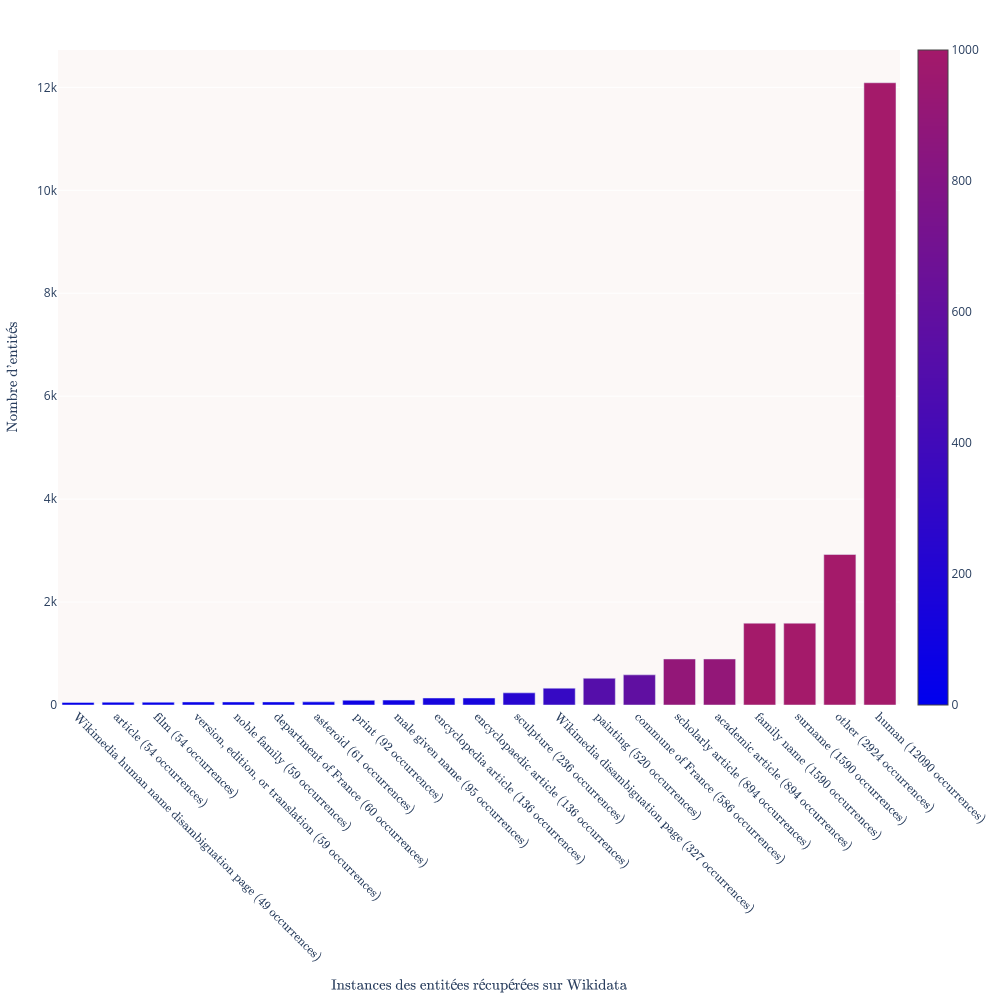
\includegraphics[width=\linewidth]{annexes/fig_wikidata_instances.png}
	\caption Occurrences des différentes catégories auxquelles appartiennent les entités \wkd{} liées avec les entrées de catalogues
	\label{appendix:wikidata_instances}
\end{figure}
\end{document}
